\documentclass{article}

% Language setting
% Replace `english' with e.g. `spanish' to change the document language
\usepackage[english]{babel}

% Set page size and margins
% Replace `letterpaper' with`a4paper' for UK/EU standard size
\usepackage[letterpaper,top=2cm,bottom=2cm,left=3cm,right=3cm,marginparwidth=1.75cm]{geometry}

% Useful packages
\usepackage{amsmath}
\usepackage{graphicx}
\usepackage[colorlinks=true, allcolors=blue]{hyperref}

\title{Elliptic Curves and the Nagell-Lutz theorem:\\a guided reinvention}
\author{Samuel Dauncey}

\begin{document}
\maketitle

\begin{abstract}
    
"Number theory has an annoying habit: the field produces, without effort, innumerable problems which have a sweet, innocent air about them, tempting flowers; and yet... number theory swarms with bugs, waiting to bite the tempted flower-lovers who, once bitten, are inspired to excesses of effort!" - Barry Mazur
\end{abstract}

\section{Introduction and Motivation}

\subsection{An innocent-looking problem}

Suppose one wanted to find all solutions to the polynomial equation:\\

$3 X^3 +  2 X Y^2 + 2 Y^3 = Z^3$ \quad For integers $X$, $Y$ and $Z$. \\

 One may realise that, given a solution; say $(X, Y, Z) = (1, 2, 3)$, one can see that we can generate infintely many more solutions $(X, Y, Z) = (2, 4, 6), \; (3, 6, 9), \; \dots \; (n, 2n, 3n) \; \dots $. This property of our equation is special, it is called \emph{homogeneity} and stems from the fact that if we sum up the powers of $X$, $Y$ and $Z$ in each of the terms of our equation, we get the same integer (in this case, three). \\
 
 Finding solutions to homogeneous equations is of special importance to number theorists, examples including the Fermat equation $X^m + Y^m = Z^m$. \\
 
 In essence, we can think of each of these infinite sets of solutions as all part of the same solution, and we can see that, if we view our solutions as coordinates in $R^3$, each one of our infinite sets of solutions can be viewed as a line going through the origin and and a point with integer coordinates. Dividing our original equation by $Z$, we can see that our problem is equivalent to finding the rational solutions to the equation:\\
 
 $3x^3 + 2xy + 2y^3 = 1$\\
 
With rational solution $(x, y) = (\frac{m}{n}, \frac{p}{q})$ being converted into $(X, Y, Z) = (m, p, nq)$ and integer solution $(X, Y, Z)$ being converted into $(\frac{X}{Z}, \frac{Y}{Z})$. However, note that this conversion isn't well-defined when $Z = 0$, so we still have to consider the integer solutions to $3 X^3 +  2 X Y^2 + 2 Y^3 = 0$. However; as this is also a homogeneous polynomial equation, we can repeat our process, this time by dividing by $Y$ to see we want to find solutions to: \\

$3 x^3 + 2 x + 2 = 0$ \quad for rational $x$ and $X^3 = 0$ for integer $X$\\

Hence, we can see that there is a one-to-one correspondence between the "lines" of integer solutions to $3 X^3 +  2 X Y^2 + 2 Y^3 = Z^3$ and rational solutions to  $3x^3 + 2xy + y^3 = 1$, \quad $3 x^3 + 2 x + 2 = 0$, and $X^3 = 0$. Thinking back to our visualisation of our solutions to our integer equation as lines, we can see that our first division resembles looking at the intersection of the plane $Z = 1$ and our solution lines, and the fact that we could recursively apply this procedure is a hint that the \emph{projective space} we are working in has some kind of recursive structure.

Now, we can trivially solve $X^3 = 0 $ to see that $X = 0$ is the only solution (corresponding to the solution $(X, Y, Z) = (0, 0, 0)$). Slightly more difficult is the rational solutions to $3x^3 + 2 x + 2 = 0$; Gauss's Lemma tells us that any solution in it's lowest terms $x = \frac{m}{n}$ must have $m$ dividing $2$ and $n$ dividing $3$, however we can see that the only candidates this leaves, $x = +-\frac{2}{3}$ do not solve the equation; so we have no solutions of the form $(X, Y, 0)$ with non-zero $Y$. Hence, we can see that the only thing stopping us from solving our starting problem is finding all the rational solutions to  $3x^3 + 2xy + y^3 = 1$; unfortunately, this turns out to be alot harder. \\

These solutions form an \emph{algebraic curve} when visualised in the $x,y-$plane, and through analysing this curve geometrically we will be able to get some description of our solution.\\

Note that, given two points $(x_1, y_1)$ and $(x_2, y_2)$ on a degree-3 algebraic curve defined by $f(x, y) = 0$, we can find a third point $(x_3, y_3)$ on the curve by projecting a line $\alpha x + \beta y + \gamma = 0$ through them and looking at the intersection with the curve (in general*). On top of this, when we solve these simultaneous equations by eliminating one variable we get two cubics for the $x$ and $y$ coordinates, $a_3 x^3 + a_2 x^2 + a_1 x + a_0 = 0$ , \quad $b_3 y^3 + b_2 y^2 + b_1 y + b_0 = 0$. We know that the sums $x_1 + x_2 + x_3 = -\frac{a_2}{a_3}$ and $y_1 + y_2 + y_3 = -\frac{b_2}{b_3}$ are satisfied; so if $x_1$, $x_2$ and our coefficients are in some field $F$, $x_3$ must also be in $F$; and likewise for our $y$ coordinates, this means that, given a pair of rational solutions we can get another rational solution by projecting a line.

* the case where $a_3$ or $b_3$ are zero corresponds to the case where our line meets our curve asymptotically, or "at infinity", and we will see more about this when we go into projective geometry.
\\ 

The first theorem we will prove is the Mordell-Wiel theorem, which tells us that we can take a finite set of rational points on our curve and, by projecting lines through them, can get every other rational point on our curve.\\

- explanation of Nagell-Lutz using only the line function:\\
Points of finite order are precisely those that eventually loop if you continually apply $P \mapsto P*P$

The Nagell-Lutz theorem gives us a set of criteria which we can use to build an algorithm for all of the rational points that form "cycles" through our operation of addition.\\

\subsection{Why cubic plane curves?}

one variable:

-pretty much fully solved?

two variables:

- degrees 1 and 2 solved

- degree 3 much harder (not all questions answered)

three variables:

- ???

Yuri Matiyasevich's negative solution to Hilbert's tenth problem: no algorithm (including the algorithm of all human mathematicians) will be able to determine whether or not a given diophantine equation has solutions.

\subsection{Assumed prior knowledge}

- Algebra: knowledge of a group, ring and field

\newpage

\section{Projective geometry}

\subsection{Homogeneous Coordinates}

In the introduction section, I hinted at the idea that we can think of linearly related solutions, such as $(1, 2, 3)$ and $(2, 4, 6)$ to our homogeneous equation  as one line in $R^3$ and we can make this rigorous by defining a new kind of space. We kind of already did this when we divided by $Z$, but this feels unnatural because it is breaking the symmetry of our equation between $X$, $Y$ and $Z$. We will see later that this kind of space is called \emph{projective space} and when we do geometry on this space it is called \emph{projective geometry}, hence the name of this section.\\

We want to define a \emph{point} such that all the solutions $(t, 2t, 3t)$ are considered to be the same, just as when we divide through by $Z$ so it makes sense to say a point in projective space as a ratio between the X, Y and Z coordinates, :\\

We denote $P = [X : Y : Z] \in P_R^2$ for real numbers $X$, $Y$ and $Z$ which are called the \emph{homogeneous} coordinates of $P$;\\

where two points are said to be equal, ie $[X : Y : Z] = [X' : Y' : Z']$ if and only if we can find a $t \in R$ satisfying $X = tX', Y =  tY'$ and $Z = tZ'$\\

Unfortunately, this on it's own is not a well-defined equivalence relation; every point is equal to $[0 : 0 : 0]$. To fix this, we simply ban this point and say if  $[X : Y : Z] \in P_R^2$  then one of $X$, $Y$ and $Z$ is non-zero. It is relatively straightforward to now mentally check that this definition of equality satisfies reflexivity, symmetry and transitivity.\\

Note that, if you view the homogeneous coordinates $X$, $Y$ and $Z$ as a point $(X, Y, Z)$ in $R^3$ then our \emph{points} in $P_R^2$ (the equivalence classes of coordinates which give equal points) can be visualised as \emph{lines} going through the origin in $R^3$. Hence, it makes intuitive sense that our \emph{lines} in $P_R^2$ could be visualised as \emph{planes} containing the origin in $R^3$. This intuition gives us the definition of a line in $P_R^2$:\\

A line in $P_R^2$ is the set of points $[X : Y : Z]$ where $AX + BY + CZ = 0$ for some fixed $A$, $B$ and $C$. \\

Note our definition of a line is well defined as  $AX + BY + CZ = 0$ iff  $A(tX) + B(tY) + C(tZ) = 0$. This geometrical intuition gives us an interesting property of lines in $P_R^2$: \\

Two distinct lines in $P_R^2$ intersect at exactly one point. For example, say we have two lines $AX + BY + CZ = 0$ and $\Bar{A}X + \bar{B}Y + \bar{C}Z = 0$. We can solve these equations simultaneously by putting them in a matrix-vector product:\\

$$ \begin{bmatrix}
A & B & C \\
\Bar{A} & \Bar{B} & \Bar{C} 
\end{bmatrix} 
\begin{bmatrix}
X \\
Y \\
Z \\
\end{bmatrix} 
= \vec{0}
$$

From this we can see that, if the two lines are distinct, then $A  B  C$ and
$\Bar{A}  \Bar{B}  \Bar{C} $ will be linearly independent, as if they weren't, we would be able to reduce their defining equations onto each other. Hence our matrix will have rank 2 and so by the rank-nullity theorem we will have one linearly independent solution for $X$, $Y$ and $Z$, corresponding to our point of intersection in $P_R^2$. This property of lines in $P_R^2$ is different to, say, $R^2$, where parallel lines intersect nowhere.

- projecting onto a plane (sphere doesn't work because of rational to rational mapping :( )
When we divided by $Z$ in our introduction, we took each point in $P_R^2$ and mapped it to a point in $R^2$, barring the points where the $Z$ coordinate was $0$. The obvious way to map points in $P_R^2$ onto a surface is to look at projecting them onto the unit sphere, For example mapping $[1 : 2 : 3]$ to the point $(,,)$. The problem with this approach is that this takes a point with rational coordinates and maps it to a point without rational coordinates; meaning it isn't very useful for us. Instead, we have to suffice by projecting our projective plane onto a flat screen.

- recursive definition

- General fields
 Note that in this section I used the real numbers, $R$ as the field that we were working over. However, the proofs used no special properties about the real numbers, hence we could replace $R$ with any field $F$ and get the same results. In general, we call $P_F^2$ the \emph{projective plane over the field} $F$,  alot of algebraic geometry is concerned with $P_C^2$ for instance, however for us it suffices to know that $P_Q^2$ is well defined.

\subsection{Projective Transformations}

\subsection{Transforming Cubic Curves}

\subsection{Groups over Cubic Curves}

Let $C(F)$ be a cubic curve working in some field $F$

As we sa:

define $P * Q \in C(F)$ to be the third point on $C(F)$,

have $P * Q = Q * P$

and $(P * Q) * Q = P$

Is $(C(F), *)$ a group? Unfortunately not; it is not hard to mentally verify that a unique identity element doesn't exist and that associativity won't hold.

For three points, $P$, $Q$ and $R$ on our curve $C$ Write $P - Q - R$ to mean these three points are colinear, this notation helps us clear up the fact that these six statements are equivalent:

$P * Q = R, P * Q = R, P * R = Q,  Q * R = P$

if $A - B - C$ and $D - E - F$ and $A - D - G$ and $B - E - H$

then $C * F = G * H$

If we slightly abuse our new notation, our theorem becomes:

if
$
\\
A - B - C \\
D - E - F \\
H - I
$\\
then, for some $J \in C(F)$:
$
\\
A - B - C \\
D - E - F \\
H - I - J
$

Although the notation makes this look intuitive, it is not at all obvious. 
Why should the line defined by $C$ and $F$ and the line defined by $H$ and $J$ intersect with the curve at the same point? 

Three cubic curves that meet at eight points $P_1 \dots P_8$ will also all meet at a ninth point $P_9$.

let v be the vector:

$
\begin{bmatrix}
X^3 \\
Y^3 \\
Z^3 \\
\end{bmatrix} 
$

-why is the group law the way it is?

- show ((A * B) * O) * C = A * ((B * C) * O) ?

therefore, if A + B = (A * B) * O then (A + B) + C = A + (B + C)

\newpage

\section{The Mordell-Wiel theorem (For elliptic curves)}

\newpage

\section{The Nagell-Lutz theorem}

\subsection{General idea and motivation}

-knowledge and familiarity with the concepts of rings asssumed\\

The Mordell-Wiel theorem gave us information about the structure of the group of rational points; however the problem of finding the rank or the generating set for some curve $C$ is still not fully solved. Thankfully, the other component of our group, the torsion subgroup, is much better understood, and in the following chapter we will go through a theorem that fully describes how to find all of it's points for any given curve C: the Nagell-Lutz theorem.\\

In general, points seem to increase their "complexity" when we add them, for instance, in our proof of the Mordell-Wiel theorem, we showed that the amount of points under some bound of the complexity measure of height was finite, and we could find a bound that contains all of the generating elements. This means that, if P is some generating element then the height of P must increase without bound, ie the sequence $h(nP)$ for natural $n$ is unbounded. This is in contrast to our points in the torsion group, where $h(nP)$ is periodic and therefore must be bounded. Hence, it seems like a good method to find the torsion points of our curve would be to look for points for which $h(nP)$ is bounded.\\

In fact, the description which the Nagell-Lutz theorem gives tells us that, if our curve has integer coefficients, then all of it's rational torsion points must have integer coefficients; ie if $T$ is the torsion subgroup then $T \subseteq C(Z)$. This is a strange and surprising result, and until we go through some of the basic lemmas of the proof, it is hard to intuitively explain why we would expect this to be the case. One thing we can see is that the complexity measure of height won't work for our proof: it is impossible to take $h(r)$ for some rational number $r \in Q$ and determine whether or not $r$ is an integer. At first, this may not seem like a big deal, however we will see later that it is not tricky to protectively transform \emph{any} elliptic curve into an elliptic curve with integer coordinates, and therefore by extension, \emph{any} cubic curve into an elliptic curve with integer coordinates.\\

The for some rational $r \in Q$ p-adic order of $r$, $ord_p(r)$ is defined as the value of the power of the prime $p$ when $p$ is completely "factored out" of $r$; ie, we can uniquely write:\\

$r = \frac{m}{n}p^v$ such that $p$, $m$ and $n$ are all coprime integers, then $ord_p(r) = v$\\

by convention, we define $ord_p(0) = \infty$ as in a sense $p$ divides $0$ infinitely\\

Knowledge of p-adic numbers is not necessary to understand the proof, however it does add to the intuitions one may have. This complexity measure has the nice property that $r$ is an integer if and only if $ord_p(r) \geq 0$ for all primes $p$, making it more suitable for the theorem that we are going to prove. \\

There are some other nice facts about p-adic order that one can mentally verify:\\

for all $q, r \in Q$:\\

- $ord_p(qr) = ord_p(q) + ord_p(r)$\\

- if $ord_p(q) = ord_p(r)$ then $ord_p(q + r)  \geq ord_p(q)$ or $ord_p(r)$\\

- if $ord_p(q) > ord_p(r)$ then $ord_p(q + r) = ord_p(r)$\\

- in general, $ord_p(q + r) \geq min(ord_p(q)$, $ord_p(r))$\\

We still don't have a measure that we can apply to points on $C(Q)$ just yet, but we can use these facts to prove a theorem about integer-coefficiented polynomials:\\

if $f(x) = x^n + c_{n-1}x^{n-1} + c_{n-2}x^{n-2} + \dots c_1 x + c_0$ is an integer coefficiented-polynomial, then for all $x \in Q$ with $ord_p(x) < 0$: $ord_p(f(x)) = n \ ord_p(x)$\\

The proof is relatively simple:

first, note that $ord_p(c_k x^k) = ord_p(c_k) + k \ ord_p(x)$ and that, as $f$ has integer coefficients, $ord_p(c_k) \geq 0$ hence $ord_p(c_k x^k) \geq k \ ord_p(x)$. However, as $ord_p(x) < 0$, $k \ ord_p(x) > n \ ord_p(x)$ for $k > n$. Hence we can see that $ord_p(c_k x^k) > ord_p(x^n)$ so our $x^n$ term will "eat" all the terms to the right of it:\\

$ord_p(x^n) = ord_p(x^n + c_{n-1}x^{n-1}) = ord_p(x^n + c_{n-1}x^{n-1} + c_{n-2}x^{n-2}) = \dots = ord_p(f(x))$\\


Thinking about this with respect to elliptic curves naturally leads us to the following corollary:\\

Let $C$ be an elliptic curve defined by $y^2 = f(x)$ for some integer coefficiented cubic $f$; Then, for all points $P = (x_P, y_P) \in C(Q)$ and all primes p; either:\\

$ord_p(x_P) \geq 0$ \quad and \quad  $ord_p(y_P) \geq 0$ \\

or \quad $ 2 \ ord_p(y_P) = 3 \ ord_p(x_P)$\\

This is not too tricky to see:\\

if \quad $ord_p(y_P) < 0$ \quad then \quad $ord_p(f(x_P)) < 0$ \quad so \quad $ord_p(x_P) < 0$

and if \quad $ord_p(x_P) < 0$ \quad then \quad $3 \ ord_p(x_P) = ord_p(f(x_P)) = ord_p(y_P^2) = 2 \ ord_p(y_P)$\\

Hence, if $ord_p(x_P) < 0$ or $ord_p(y_P) < 0$ we should be able to find an integer $v > 0$ such that: $ord_p(x_p) = -2v$ and $ord_p(y_P) = -3v$\\

Applying this with all primes p tells us that $x_P$ and $y_P$ are of the form:

$x_P = \frac{m}{e^2}$ \quad and \quad $y_P = \frac{n}{e^3}$ for some integers $m$, $n$ and $e$

This becomes tricky to analyse; however we are nearing in on the complexity measure we want to use for our points. Namely, if we define $t(P) = \frac{x_P}{y_P}$ then we see that, using the definition of $v$ above, $ord_p(t(P)) = ord_p(x_p) - ord_p(y_P) = v$. \\

Hence, if we can prove $ord_p(t(P)) \geq 0$ then, it cannot be the case that $ord_p(x_P) < 0$ or $ord_p(y_P) < 0$. hence we can prove $P$ has integer coordinates by proving  $ord_p(t(P)) \geq 0$ for all primes $p$\\


Note that $P \in C(p^v)$ implies $t(P) \in p^v R$ but not the other way round; take for instance this case where $p = 2$:

$P = (2, 3)$ is on the curve $y^2 = x^3 - x + 3$ and we can see $t(P) = \frac{2}{3} \in 2^1 R$ but $P \notin C(2^1)$ 



\subsection{Examining t(P + Q)}

Let R be the ring of integers with p-adic order greater than or equal to 0 (ie, the integers which have powers of p only in their numerator if at all):\\

$R = \{r \in Q \; | \; ord_p(r) \geq 0\}$\\

Then we can see that our ideals of $R$ generated by $p^v$ are precisely the sets of rational numbers with p-adic order greater than than or equal to $v$:\\

$p^vR = \{r \in Q \; | \; ord_p(r) \geq v\}$\\

Let $P$ and $Q$ both be in $C(p^v)$ for some $v$. We wish to study the p-adic order of the coordinates of $P + Q$ to see if we get anything interesting.

First, we will apply a protective transformation (what is the rationale?); and label our new coordinates $(t, s)$

$(x, y) \mapsto (t, s)$ such that:

$t = \frac{x}{y}$ and $s = \frac{1}{y}$ \\

The important thing to note here is that $P \in C(p^v)$ iff $ord_p(x_P) = -2v$ and $ord_p(y_P) = -3v$ iff $ord_p(t_P) = v$ and $ord_p(s_P) = 3v$; so this transformation doesn't loose any information about $P$ being in $C(p^v)$\\

This transformation is it's own inverse, so $x$ and $y$ are given by:\\

$x = \frac{t}{s}, y = \frac{1}{s}$\\

Plugging these into our curve's equation gives:\\

$\frac{1}{s^2} = \frac{t^3}{s^3} + a \frac{t^2}{s^2} + b \frac{t}{s} + c$\\

hence:\\

$s = t^3 + a t^2 s + b t s^2 + c s^3$\\

Now, to add $(t_P, s_P)$ and $(t_Q, s_Q)$ on our curve we simply follow the procedure for a standard cubic curve.

First, we find the line going through $t_P$ and $t_Q$:

$s = \alpha t + \beta$ with $\alpha = \frac{s_P - s_Q}{t_P - t_Q}$ and $\beta = s_P - \alpha t_P$ \\

Then, we simultaneously solve the line equation and the curve equation to find the third intersection point:

$\alpha t + \beta = t^3 + a t^2 (\alpha t + \beta) + b t (\alpha t + \beta)^2 + c (\alpha t + \beta)^3$\\

Collecting terms gives:\\

$0 = k_3 t^3 + k_2 t^2 + k_1 t + k_0$\\

where $k_3 = 1 + a \alpha + b \alpha^2 + c \alpha^3$ and $k_2 = a \beta + + 2 b \alpha \beta + 3c \alpha^2 \beta$\\

hence: $t_P + t_Q + t_{P*Q} = -\frac{k_2}{k_3}$\\

Note that in our projective transformation the zero point was mapped to the origin and our curve is symmetric about the line $t + s = 0$ as if $(t, s)$ is on our curve then $(-t, -s)$ will also be on our curve. Combining these pieces of information, it is not too tricky to see that $(t_{P + Q}, s_{P + Q}) = (-t_{P * Q}, -s_{P * Q})$, hence we have that:\\

$t_P + t_Q - t_{P+Q} = -\frac{k_2}{k_3}$\\

After this rather laborious bit of algebra, we can see a few things pop out at us: namely, if we can prove that $-\frac{k_2}{k_3} \in p^v R$ then we can prove that $t_{P+Q} \in p^v R$, strongly suggesting that $C(p^v)$ is a subgroup. Unfortunately, to get more information about $-\frac{k_2}{k_3}$ we must first go back and examine $\alpha$ and $\beta$. \\

As $s_P$ and $s_Q$ are in $p^{3v}R$ and $t_P$ and $t_Q$ are only in $p^v R$ it seems intuitive that $\alpha \in p^{2v}R$, however the preceding information alone doesn't give us enough information to \emph{prove} this. We need to also use the information that links $s_P$ with $t_P$ and $s_Q$ with $t_Q$; namely that they satisfy the cubic equation for our curve. Examining the top part of our fraction for $\alpha$, , $s_P - s_Q$, gives:

\begin{align*} 
s_P - s_Q &= t_P^3 - t_Q^3 + a \; t_P^2 s_P - a \; t_P^2 s_P + b \; t_P s_P^2 - b \; t_Q s_Q^2 + c \; s_p^3 - c \; s_Q^3 \\
&= t_P^3 - t_Q^3 \\
& \quad + a(t_P^2 s_P - t_P^2 s_Q + t_P^2 s_Q - t_Q^2 s_Q) \\
& \quad + b(t_P s_P^2 - t_Q s_P^2 + t_Q s_P^2 - t_Q s_Q^2) \\
& \quad + c(s_P^3 - s_Q^3) \\
&= (t_P - t_Q)(t_P^2 + t_P t_Q + t_Q^2) \\
& \quad + a(s_P - s_Q)t_P^2 + a(t_P - t_Q)(t_P + t_Q)s_Q \\
& \quad + b(t_P - t_Q)s_P^2 + b(s_P - s_Q)(s_P + s_Q)t_Q \\
& \quad + c(s_P - s_Q)(s_P^2 + s_P s_Q + s_Q ^2)
\end{align*} 


Factoring out $s_P - s_Q$ and $t_P - t_Q$ gives:\\

$(1 - A)(s_P - s_Q) = B(t_P - t_Q)$ where $A = a t_P^2 + b(s_P + s_Q)t_Q + c(s_P ^2 s_p s_Q + s_Q^2)$ 

and $B = (t_P^2 + t_P t_Q + t_Q^2) + a (t_P + t_Q)s_Q + b s_p^2$\\

Hence: $\alpha = \frac{s_P - s_Q}{t_P - t_Q} = \frac{B}{1 - A}$\\

Now, we can see that $B \in p^{2v}R$ and $A \in p^{2v} R$ from the fact that they are the sums of terms in these ideals. Hence, $ord_p(A) \geq 2v \geq 0 = ord_p(1)$ so $ord_p(1 - A) = 0$, meaning that we can conclude that $\alpha = \frac{B}{1 - A} \in p^{2v}R$


- prove that if $t(P) \in p^v R$ and $t(Q) \in p^v R$ then $t(P) + t(Q) + t(P * Q) \in p^{3v}R$ \\

- $t(P * Q) = - t(P + Q)$\\

- Hence $t(P) + t(Q) \equiv t(P + Q)  \quad (\bmod{p^{3v}R}$)\\

\newpage

\subsection{Finishing off the proof}

Let $p$ be any prime number\\

Let $P \in C(Q)$ be a point of order $m$ with $m \neq 1$. We will show $P \notin C(p)$ \\

First, we need to factor most (or all) of the powers of $p$ in $m$ so that they don't interfere with our proof (We will see later why this is necessary).\\

It is not hard to see that for any $m \neq 1$ we can find a $\bar{m} \neq 1$ that divides $m$ and has at most one factor of $p$. For instance, if $m$ has no factors of $p$ we can pick $\bar{m} = m$ and otherwise we can pick $\bar{m} = \frac{m}{p^k}$

Now, let $P' = \frac{m}{\bar{m}} P$. We can see it suffices to prove $P' \notin C(p)$ as $C(p)$ is a subgroup\\

Let $v$ be the unique natural number such that: $P' \in C(p^v)$ but $P' \notin C(p^{v+1})$ \\

if $v = 0$, we are done as $P' \notin C(p)$. Hence we are restricted to examining the case where $v > 0$, and in this case we can deduce that $ord_p(t(P')) = v$ Now, we can examine $P'$ using the congruence relation:\\

first, note; $t(\bar{m}P') = t(mP) = t(0) = 0$\\

Hence, $\bar{m}t(P') \equiv t(\bar{m}P') \equiv 0 \quad (\bmod{p^{3v}R})$\\

Hence $\bar{m}t(P') \in p^{3v}R$\\

Now we see why we chose to examine $P'$ rather than $P$: if we got to this stage with $P$, we would not be able to say much in general as the number in front of $t(P)$ could be arbitrarily divisible by $p$, However, as $\bar{m}$ has at most one factor of p, we can say:\\

$t(P') \in p^{3v-1}R$\\

hence $ord_p(t(P)) \geq 3v - 1$\\

however, we know $ord_p(t(P)) = v$\\

hence: $v \geq 3v - 1$\\

So we are forced to conclude $v = 0$, which is a contradiction as we were restricted to the case $v > 0$.

Hence, for all points of finite order $P$ with $mP = 0$; either:

- $m = 1$ in which case $P = 0$

- $m \neq 1$ in which case $P \notin C(p)$ for all primes $p$, so $P$ must have integer coordinates



\subsection{Further constricting the set of torsion candidates}

Let $P \neq 0$ be a point of finite order. We have proved that if $(x, y) = P$ then $x$ and $y$ must be integers; however this unfortunately still gives us an infinite search space of possible candidates of points that could be torsion points on the curve. Thankfully, it is not too tricky to restrict this set to a finite set.\\

First, we know that as $P$ is on the curve, \\

$y^2 = f(x) = x^3 + a x^2 + b x + c$\\

equivalently,\\

$y^2 - c = x(x^2 + a x + b)$\\

Hence, we can see that for any candidate $y$, $x$ must divide $y^2 - c$ to give an integer point on the curve. So all we need to find is a finite set of candidate $y$ values; which is described by the following lemma:\\

If $P = (x, y)$ is a point of finite order then $y$ divides the discriminant of $f$\\

\subsection{An algorithm for generating the set of torsion candidates}

\newpage

\section{Some examples to get started}

\subsection{How to create Sections and Subsections}

Simply use the section and subsection commands, as in this example document! With Overleaf, all the formatting and numbering is handled automatically according to the template you've chosen. If you're using Rich Text mode, you can also create new section and subsections via the buttons in the editor toolbar.

\subsection{How to include Figures}

First you have to upload the image file from your computer using the upload link in the file-tree menu. Then use the include graphics command to include it in your document. Use the figure environment and the caption command to add a number and a caption to your figure. See the code for Figure \ref{fig:frog} in this section for an example.

Note that your figure will automatically be placed in the most appropriate place for it, given the surrounding text and taking into account other figures or tables that may be close by. You can find out more about adding images to your documents in this help article on \href{https://www.overleaf.com/learn/how-to/Including_images_on_Overleaf}{including images on Overleaf}.
\newpage
\begin{figure}
\centering
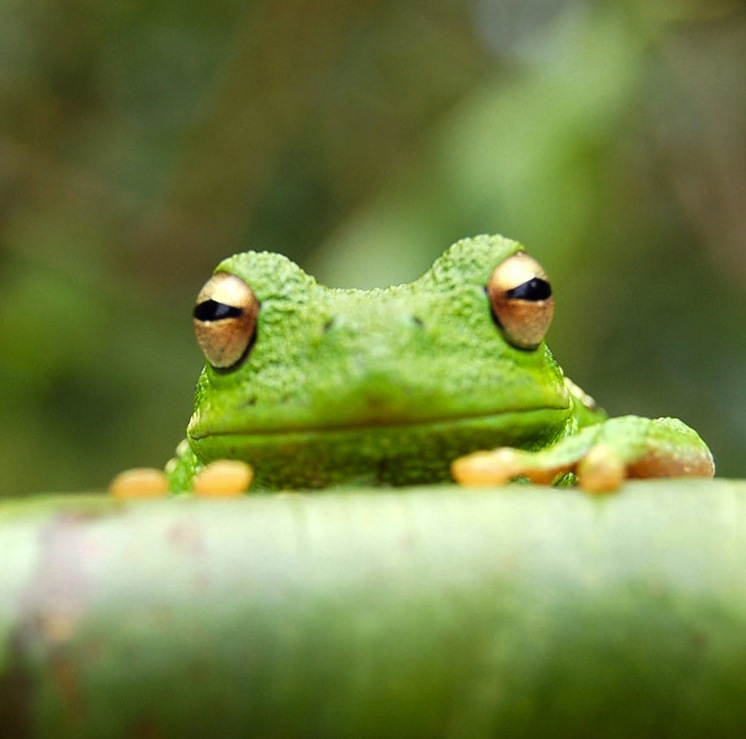
\includegraphics[width=0.3\textwidth]{frog.jpg}
\caption{\label{fig:frog}This frog was uploaded via the file-tree menu.}
\end{figure}

\subsection{How to add Tables}

Use the table and tabular environments for basic tables --- see Table~\ref{tab:widgets}, for example. For more information, please see this help article on \href{https://www.overleaf.com/learn/latex/tables}{tables}. 

\begin{table}
\centering
\begin{tabular}{l|r}
Item & Quantity \\\hline
Widgets & 42 \\
Gadgets & 13
\end{tabular}
\caption{\label{tab:widgets}An example table.}
\end{table}

\subsection{How to add Comments and Track Changes}

Comments can be added to your project by highlighting some text and clicking ``Add comment'' in the top right of the editor pane. To view existing comments, click on the Review menu in the toolbar above. To reply to a comment, click on the Reply button in the lower right corner of the comment. You can close the Review pane by clicking its name on the toolbar when you're done reviewing for the time being.

Track changes are available on all our \href{https://www.overleaf.com/user/subscription/plans}{premium plans}, and can be toggled on or off using the option at the top of the Review pane. Track changes allow you to keep track of every change made to the document, along with the person making the change. 

\subsection{How to add Lists}

You can make lists with automatic numbering \dots

\begin{enumerate}
\item Like this,
\item and like this.
\end{enumerate}
\dots or bullet points \dots
\begin{itemize}
\item Like this,
\item and like this.
\end{itemize}

\subsection{How to write Mathematics}

\LaTeX{} is great at typesetting mathematics. Let $X_1, X_2, \ldots, X_n$ be a sequence of independent and identically distributed random variables with $\text{E}[X_i] = \mu$ and $\text{Var}[X_i] = \sigma^2 < \infty$, and let
\[S_n = \frac{X_1 + X_2 + \cdots + X_n}{n}
      = \frac{1}{n}\sum_{i}^{n} X_i\]
denote their mean. Then as $n$ approaches infinity, the random variables $\sqrt{n}(S_n - \mu)$ converge in distribution to a normal $\mathcal{N}(0, \sigma^2)$.


\subsection{How to change the margins and paper size}

Usually the template you're using will have the page margins and paper size set correctly for that use-case. For example, if you're using a journal article template provided by the journal publisher, that template will be formatted according to their requirements. In these cases, it's best not to alter the margins directly.

If however you're using a more general template, such as this one, and would like to alter the margins, a common way to do so is via the geometry package. You can find the geometry package loaded in the preamble at the top of this example file, and if you'd like to learn more about how to adjust the settings, please visit this help article on \href{https://www.overleaf.com/learn/latex/page_size_and_margins}{page size and margins}.

\subsection{How to change the document language and spell check settings}

Overleaf supports many different languages, including multiple different languages within one document. 

To configure the document language, simply edit the option provided to the babel package in the preamble at the top of this example project. To learn more about the different options, please visit this help article on \href{https://www.overleaf.com/learn/latex/International_language_support}{international language support}.

To change the spell check language, simply open the Overleaf menu at the top left of the editor window, scroll down to the spell check setting, and adjust accordingly.

\subsection{How to add Citations and a References List}

You can simply upload a \verb|.bib| file containing your BibTeX entries, created with a tool such as JabRef. You can then cite entries from it, like this: \cite{greenwade93}. Just remember to specify a bibliography style, as well as the filename of the \verb|.bib|. You can find a \href{https://www.overleaf.com/help/97-how-to-include-a-bibliography-using-bibtex}{video tutorial here} to learn more about BibTeX.

If you have an \href{https://www.overleaf.com/user/subscription/plans}{upgraded account}, you can also import your Mendeley or Zotero library directly as a \verb|.bib| file, via the upload menu in the file-tree.

\subsection{Good luck!}

We hope you find Overleaf useful, and do take a look at our \href{https://www.overleaf.com/learn}{help library} for more tutorials and user guides! Please also let us know if you have any feedback using the Contact Us link at the bottom of the Overleaf menu --- or use the contact form at \url{https://www.overleaf.com/contact}.

\bibliographystyle{alpha}
\bibliography{sample}

\end{document}